\chapter{Software involucrado en el proyecto} \label{chap:SW}
\hrule
\vspace{3mm}

    En este capítulo se hace una descripción detallada del \ingles{software} involucrado en este proyecto. Primeramente se hace un repaso de la estructura de directorios, que es característica y viene previamente marcada por el software utilizado. Una vez explicado se pasará a describir las diferentes librerías que se han desarrollado (sección \ref{sec:SW:lib}) y del directorio de fuentes principal SRC (sección \ref{sec:SW:src}). Se deja para una sección posterior la interacción e integración de estos objetos así como una explicación más detallada del flujo de la información, funcionamiento del sistema como ejemplos de uso (sección \ref{sec:SW:interacion_informacion_proced}). Finalmente se exponen los test realizados sobre el software (sección \ref{sec:SW:test}) así como la gestión de la complejidad (sección \ref{sec:SW:gestion_complejidad}) del proyecto.
    \\ 

    Para el desarrollo y test del software se ha utilizado el editor \glosario{Atom} ampliando su funcionalidad con el paquete \glosario{PlatformIO}, que expande las capacidades del editor base para permitir trabajar con diferentes placas \completar, entre ellas las de la gama de \glosario{Arduino}.
    \\ 
    
    La elección de esta herramienta conlleva un formato en el árbol de directorios en los que se separa el código debido a la forma que tiene de compilar y lincar los diferentes ficheros. De esta manera y para mantener el orden los ficheros de código se separan en distintos directorios:
    
    \begin{itemize}
    	\item lib: directorio donde se introducen, en carpetas, las librerías que se van a utilizar.
    	\item src: directorio donde se introduce el fichero o ficheros de código principales.
    	\item test: directorio donde se introducen los ficheros donde se codifican los test. Estos irán metidos dentro de directorios con el nombre de cada test.
    \end{itemize}
    
    Concretamente, en el caso de este proyecto, queda el siguiente árbol de directorios en el cual se han expandido hasta el nivel de ficheros en algunos casos de modo que sirvan de ejemplo:

    \lstset{language=C, breaklines=true, basicstyle=\footnotesize}
        %Introducir label y caption
        \begin{lstlisting}[frame=single]
        
     -- Sw
     |-- lib
     |   |-- debug
     |   |   | + debug.cpp
     |   |   | + debug.h
     |   |-- joint_handler
     |   |   | + joint_handler.cpp
     |   |   | + joint_handler.h
     |   |-- joint_rha
     |   |-- rha_types
     |   |-- robot_rha
     |   |-- servo_rha
     |   |-- chuck_handler
     |   |-- readme.txt
     |-- src  
     |   |-- main.cpp
     |   |-- utilities.cpp
     |   |-- utilities.h
     |-- test
     |   |-- a_test_servo_rha
     |   |   | + test_servo_rha.cpp
     |   |-- b_ttest_servo_realest_joint_rha
     |   |-- c_test_joint_handler_mock
     |-- platformio.ini
     -------
     |-- code_analysis
     |-- makeAnalysis.sh
        \end{lstlisting}
    
    En los siguientes apartados se hará un análisis detallado del contenido de estos directorios. Se desarrollan primero los ficheros con información auxiliar y posteriormente en una jerarquía desde más afuera \textcolor{pRojo}{$<$---- ¿?¿W T F?¿?} detallando luego los componentes internos.
\section{Librerías (directorio lib)} \label{sec:SW:lib}

    \subsection{debug} \label{subsec:SW:lib:debug}
        Dentro de este directorio se encuentra el fichero debug.h donde se han definido macros para \glosario{debug} de los diferentes espacios. A continuación se muestra un ejemplo de como se codifican dichas macros para hacer un seguimiento de la clase \ingles{servo\_rha} (Ver apartado \ref{subsec:SW:lib:servo_rha}).
        
        \lstset{language=C, breaklines=true, basicstyle=\footnotesize}
        %Introducir label y captio
        \begin{lstlisting}[frame=single]
        
    #ifdef DEBUG_SERVO_RHA
        #define DebugSerialSRHALn(a) {  Serial.print("[DC]  ServoRHA::"); Serial.println(a); }
        #define DebugSerialSRHALn2(a, b) {  Serial.print("[DC]  ServoRHA::"); Serial.print(a); Serial.println(b); }
        #define DebugSerialSRHALn4(a, b, c, d) {  Serial.print("[DC]  ServoRHA::"); Serial.print(a); Serial.print(b); Serial.print(c); Serial.println(d); }
    #else
        #define DebugSerialSRHALn(a)
        #define DebugSerialSRHALn2(a, b)
        #define DebugSerialSRHALn4(a, b, c, d)
    #endif
            
        \end{lstlisting}

        Como se puede apreciar estas macros utilizan la comunicación serial de \glosario{Arduino}, concretamente la función \ingles{print} y \ingles{println} de la librería \ingles{Serial} para mostrar los mensajes en un formato determinado. Además se definen de tal forma que se pueden activar o desactivar (en este mismo fichero \ingles{debug.h}) de forma que se enviarán o no los mensajes de \glosario{debug}. A través de este tipo de mensajes se puede hacer un seguimiento de la ejecución de los diferentes métodos o funciones de la librería afectada para ubicar fallos en los mismos.

        Para activar la opción de \glosario{debug} bastará con descomentar la línea correspondiente:

        \lstset{language=C, breaklines=true, basicstyle=\footnotesize}
        %Introducir label y captio
        \begin{lstlisting}[frame=single]
        
    // #define DEBUG_SERVO_RHA
    // #define DEBUG_TEST_SERVO_RHA_MOCK
    #define DEBUG_TEST_SERVO_RHA_REAL
    // #define DEBUG_CYTRON_G15_SERVO
    // #define DEBUG_TEST_CYTRON_G15_SERVO
            
        \end{lstlisting}
        
    \subsection{rha\_types} \label{subsec:SW:lib:rha_types}
        Dentro de este directorio se encuentra el fichero \ingles{rha\_types.h} donde se definen algunos tipos de datos y estructuras que se usan en el proyecto.
        \\
        
        Estas estructuras de datos se listan a continuación, pudiendo ver sus respectivos diagramas de clases en la figura \ref{fig:SW:class_diagram_TRHA}:
        
        \begin{itemize}
            \item \ingles{SpeedGoal} condensa en un solo objeto toda la información necesaria para codificar un objetivo de velocidad.
            \item \ingles{Regulator} encapsula el funcionamiento de un \glosario{Regulador-PID} estandar. Guarda los valores de las constantes así como de la integral del error para luego, pasándole error, derivada del error e integral del error en un intervalo poder devolver la salida del regulador.
            \item \ingles{Timer} codifica un temporizador (en milisegundos) de forma que se le podrá preguntar al objeto si el tiempo ya ha pasado, bloqueando o no la ejecución del programa hasta el final del tiempo.
            \item \ingles{TimerMicroseconds} hereda las características del objeto \ingles{Timer} funcionando en microsegundos.
        
        \end{itemize}
        
        \begin{figure}[H]
            \centering
            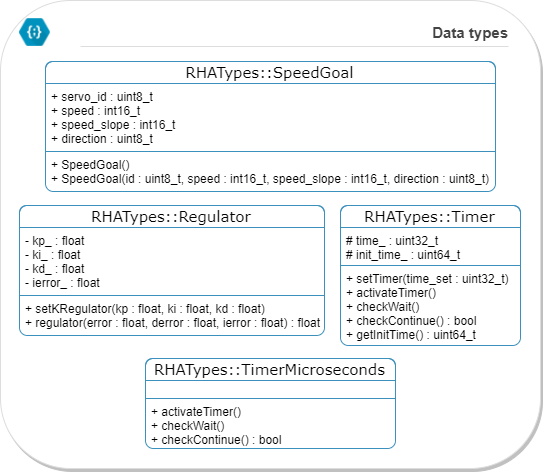
\includegraphics[width=0.8\textwidth]{figuras/SW/class_diagram_TRHA.png}   
            \caption{Estructuras de datos auxiliares}
            \label{fig:SW:class_diagram_TRHA}
        \end{figure}
        
        Se puede consultar información de más bajo nivel referente a estos tipos de datos en el Anexo \ref{app:documentacion_software} sección \completar.
    \subsection{joint\_handler} \label{subsec:SW:lib:joint_handler}
        La librería \ingles{joint\_handler} se hace cargo de generar un objeto de la clase \ingles{JointHandler} que será en encargado de gestionar la sincronización de todas las articulaciones. Este objeto es propietario de las articulaciones e implementa un método que cíclicamente sincroniza el funcionamiento de todas las articulaciones. En el objeto \ingles{JointHandler} se implementa a su vez la comunicación con los \glosarioPlural{servo}, es decir, el encapsulamiento de los paquetes de datos con la información genérica de forma que la información que se envía cumpla con el protocolo de comunicación que comparten los \glosarioPlural{servo}. Además implementa las funciones que gestionan el envío y recepción de dichos paquetes de datos.
        
        El bucle de control implementado se encarga de ir llamando una a una a todas las articulaciones para que hagan las siguientes operaciones (se puede ver representado el funcionamiento de dicho ciclo en la Figura \ref{fig:SW:joint_handler_loop}):
        \begin{enumerate}
            \item Asegurar que cada articulación actualice la información propia, compuesta por la posición recibida de la realimentación así como toda la información proveniente del servo (datos de posición, velocidad, par soportado y dirección en que se aplican, voltaje y temperatura).
            \item Llamar a cada articulación para que se realicen los cálculos correspondientes del \ingles{torque} que se enviará calculado a partir del error entre la velocidad real y deseada. Este valor queda guardado en cada servo para ser posteriormente empaquetado.
            \item Invocar a cada servo para que se adhieran al paquete de información que se va a enviar.
            \item Se enpaqueta la información a enviar a los diferentes \glosarioPlural{servo} en un mismo paquete, añadiendo posteriormente el correspondiente encabezado así como el comprobante de que el paquete se ha recibido correctamente (checksum). Una vez preparado el paquete se envía por el puerto serie.
        \end{enumerate}
        
        \begin{figure}[H]
        \centering
        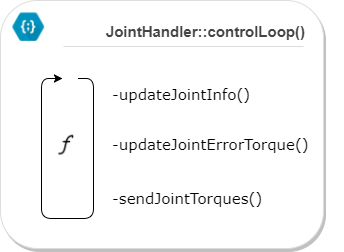
\includegraphics[width=0.45\textwidth]{figuras/SW/joint_handler_loop.png}   
        \caption{Esquema de ejecución de bucle de control de joint\_handler}
        \label{fig:SW:joint_handler_loop}
        \end{figure}
        
        Como se puede intuir es en este objeto donde realmente se implementa el lazo de control de velocidad para todos los \glosarioPlural{servo} conectados al bus. Esta serie de operaciones descrita anteriormente constituye, de forma discretizada, el lazo de control representado en la Figura \ref{fig:SW:servo_control_loop} para cada servo y asegura su correcto funcionamiento y sincronismo.
        
        \begin{figure}[H]
        \centering
        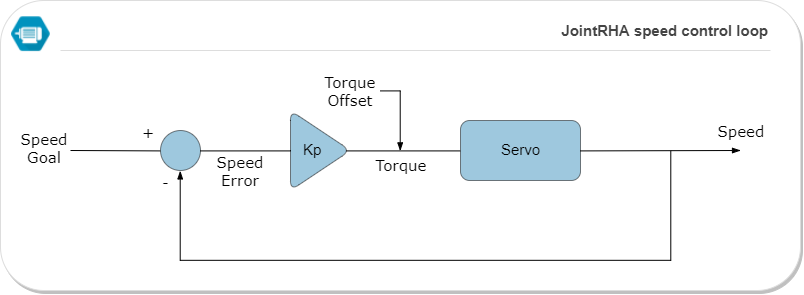
\includegraphics[width=0.85\textwidth]{figuras/SW/servo_control_loop.png}   
        \caption{Lazo de control de la velocidad del servo. Cálculos realizados por el objeto \ingles{ServoRHA}.}
        \label{fig:SW:servo_control_loop}
        \end{figure}
            
        \begin{figure}[H]
            \centering
            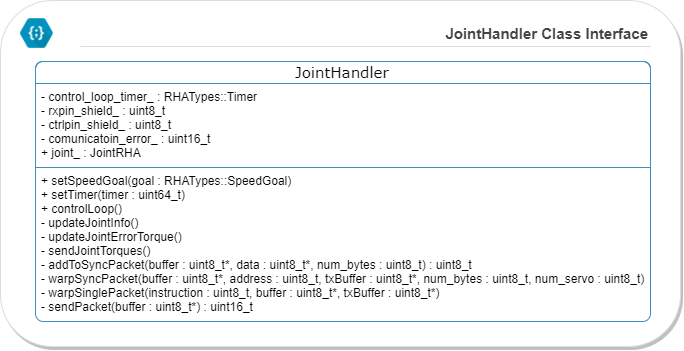
\includegraphics[width=0.95\textwidth]{figuras/SW/class_diagram_JH.png}   
            \caption{Atributos y métodos más relevantes del objeto \textit{JointHandler}}
            \label{fig:SW:class_diagram_JH}
        \end{figure}
        
        Se puede consultar información de más bajo nivel referente al objeto \ingles{JointHandler} así como a sus atributos y métodos en el Anexo \ref{app:documentacion_software} sección \completar.
    
    \subsection{joint\_rha} \label{subsec:SW:lib:joint_rha}
        La librería \ingles{joint\_rha} implementa un objeto de tipo \ingles{JointRHA} que aúna en un mismo objeto las lecturas y capacidades del objeto \ingles{ServoRHA} (explicado en la sección \ref{subsec:SW:lib:servo_rha}) junto con la realimentación de posición de la articulación en cuestión.
        
        \begin{figure}[H]
            \centering
            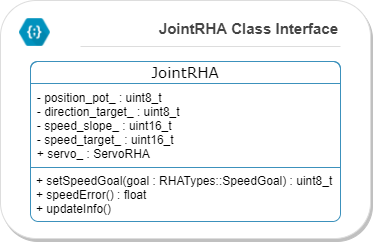
\includegraphics[width=0.5\textwidth]{figuras/SW/class_diagram_JRHA.png}   
            \caption{Atributos y métodos más relevantes del objeto \textit{JointRHA}}
            \label{fig:SW:class_diagram_JRHA}
        \end{figure}
        
        Se puede consultar información de más bajo nivel referente al objeto \ingles{JointRHA} así como a sus atributos y métodos en el Anexo \ref{app:documentacion_software} sección \completar.
        
    \subsection{servo\_rha} \label{subsec:SW:lib:servo_rha}
        La librería \ingles{servo\_rha} implementa un objeto del tipo \ingles{ServoRHA} que está encargado de gestionar toda la información referente al servo. Se encarga de encapsular la información específica a un servo en paquetes de datos a petición del objeto \ingles{JointHandler} que luego serán procesados por el mismo previo a ser enviados a través del bus. Estos paquetes se forman a partir de la información contenida en el objeto \ingles{ServoRHA}, que además de formar los paquetes a enviar almacena la información referente al servo que se recibe de los mismos. 
        \\
        
        Gestiona además una parte importante referente al lazo de control de velocidad del servo vista en el apartado \ref{subsec:SW:lib:joint_handler}. El objeto \ingles{ServoRHA} contiene los datos del regulador utilizado así como el offset a aplicar. De esta forma, recibiendo el error realiza las operaciones para calcular y empaquetar el \ingles{torque} deseado. En la Figura \ref{fig:SW:servo_control_loop_servo_part} se representa, recuadrado, la parte correspondiente del lazo de control de velocidad (representado anteriormente en la Figura \ref{fig:SW:servo_control_loop}) que efectúa el objeto en cuestión.
        \begin{figure}[H]
        \centering
        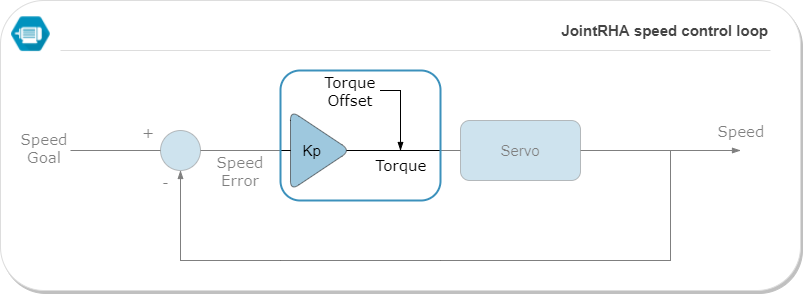
\includegraphics[width=0.85\textwidth]{figuras/SW/servo_control_loop_servo_part.png}   
        \caption{Lazo de control de la velocidad del servo. Cálculos realizados por el objeto \textit{ServoRHA}.}
        \label{fig:SW:servo_control_loop_servo_part}
        \end{figure}
        
        \begin{figure}[H]
            \centering
            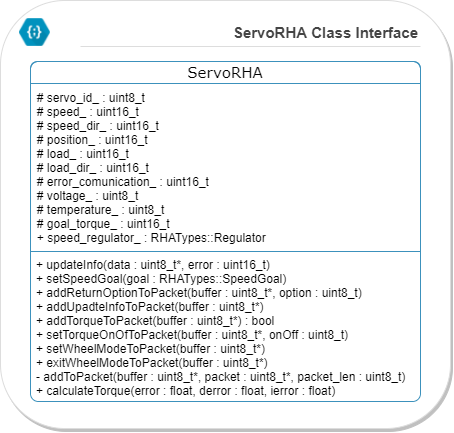
\includegraphics[width=0.65\textwidth]{figuras/SW/class_diagram_SRHA.png}   
            \caption{Atributos y métodos más relevantes del objeto \textit{ServoRHA}}
            \label{fig:SW:class_diagram_SRHA}
        \end{figure}
        
        Se puede consultar información de más bajo nivel referente al objeto \ingles{ServoRHA} así como a sus atributos y métodos en el Anexo \ref{app:documentacion_software} sección \completar.
        
    \subsection{robot\_rha} \label{subsec:SW:lib:robot_rha}
        En la librería \ingles{robot\_rha} se implementa el objeto de tipo \ingles{RobotRHA} encargado de coordinar el funcionamiento del robot. Implementa el ciclo de más alto nivel donde se actualizan los objetivos ya sean de posicion o velocidad para llamar a las funciones correspondientes que lo traducen a valores articulares que luego se ejecutan.
        \\ 
        
        Tiene diferentes modos de funcionamiento según de donde provengan los comandos a seguir:
        \begin{itemize}
            \item Control a través de un \ingles{Nunchuk} de la consola \ingles{Wii}. Se controla la velocidad del robot en sus diferentes ejes a través del joystic y los botones del mando. 
        
        \end{itemize}
        
    \subsection{chuck\_handler} \label{subsec:SW:lib:chuck_handler}
        La librería \ingles{chuck\_handler} codifica el objeto de tipo ChuckHandler que se encarga de implementar todo lo necesario para realizar lecturas del mando \ingles{Nunchuck} de la \ingles{Wii} y devolver comandos de velocidad con un periodo establecido. Se llamará al método correspondiente de forma continuada devolviendo este los valores de velocidad cuando se cumpla el tiempo mínimo establecido.
        
\section{SRC. Fichero de código principal} \label{sec:SW:src}

\section{Interacción entre objetos, flujo de la información y de procedimientos} \label{sec:SW:interacion_informacion_proced}

	Como se ha visto en los apartados anteriores (sección \ref{sec:SW:lib}) el control de la información está separado entre los diferentes objetos. Primeramente se va a detallar como se distribuye y gestiona la información para el control de velocidad, revisando como se construyen los paquetes necesarios para satisfacer los requerimientos del protocolo de comunicación de los servos.
	\\ 
	Como se ha visto es el objeto de tipo \ingles{JointRHA} el encargado de almacenar la información concreta de cada articulación. Aúna la información de la realimentación de posición del potenciómetro con la contenida en el objeto \ingles{ServoRHA} que contiene. Este último almacena la información referente al servo, tanto el estado como la acción de control de velocidad así como la próxima consigna de velocidad (traducida a par) que se va a enviar.
	\\ 
	
	La información fluye entre los diferentes objetos en forma de paquetes (vectores o arrays de \ingles{bytes}) que se van completando por el responsable de cada operación.
	\\ 

	El objeto JoingHandler es el encargado de adecuar la información al protocolo de comunicación concreto de los servos. Para ello pide a los servos la información concreta que se va a enviar a cada en cada caso. Se exponen a continuación dos ejemplos:
	\begin{enumerate}
		\item Un primer caso de lectura de información (actualizar la información de los servos)
		\item Un ejemplo de una operación de escritura (enviar una consigna de velocidad a los servos).
	\end{enumerate} 
	
	En el primer caso será el objeto \ingles{JointHandler} quien pase un paquete vacío al objeto \ingles{JointRHA} (en este caso se pretende actualizar la información del objeto \ingles{ServoRHA} por lo que se accederá al mismo directamente) con una petición de que se almacene en dicho paquete la información referente a la lectura: cuantos bytes se quieren leer y a partir de que dirección de memoria en los registros de los servos (se puede ver una tabla con todas las direcciones de memoria disponibles en los servos en el Anexo \ref{app:registros_g15}).
	\\ 
	
	De esta forma el Servo recibe un paquete vacío que rellena con la información correspondiente y lo devuelve al objeto \ingles{JointHandler}, que, a partir de esa información monta un paquete acorde con el protocolo de los servos añadiendo la cabecera correspondiente, la comprobación del error y la orden para que se realice una operación de lectura, entre otros datos.
	\\ 
	
	Una vez enviado, y tratándose de una operación de lectura se espera la respuesta por parte del servo correspondiente, en caso de ser satisfactoria (no se haya producido ningún error durante la operación) se filtra nuevamente la cabecera y demás información propia del protocolo de comunicación para volver a enviar, ahora lleno, el paquete de información con los bytes pedidos al objeto ServoRHA.
	
	\completarCon{Incluir diagrama con el flujo de información y ejemplo}
	
	El segundo caso será equivalente. El servo rellena en el \ingles{buffer} la información propia como es el ID del servo, la posición sobre la que se quiere escribir, el número de bytes a escribir y la información que se escribirá.
	\\ 
	El objeto \ingles{JointHandler} se encarga de rellenar los datos propios del protocolo añadiendo en este caso una orden de escritura en el paquete.
	\\ 
	\completarCon{Incluir diagrama con el flujo de la información y ejemplo}
	
	\completarCon{Comentar el resto del software}
	
\section{Test y verificación del software} \label{sec:SW:test}
    Como parte del proyecto se han desarrollado una serie de test para verificar el correcto funcionamiento de las diferentes librerías. El \ingles{testing} del \ingles{software} se ha utilizado como herramienta implémentandose solo en aquellos casos en que facilita la verificación y comprobación del correcto funcionamiento del código implementado. El \ingles{testing} del código no forma parte del núcleo del proyecto por lo que no se han establecido porcentajes mínimos de cobertura (cantidad de código que se está evaluando a través de las pruebas) ni objetivos mínimos. Los test son puramente funcionales desarrollándose los necesario y no forzando el desarrollo de los distintos niveles de \ingles{test}: test unitarios, test de integración y test de sistemas. \completarCon{Alguna cita que hable de los niveles de test}

    Para el desarrollo y ejecución de dichos test se ha utilizado la funcionalidad de test que viene integrada en \glosario{PlatformIO}: \glosario{PlatformIO_Test}. Esta herramienta, permite definir una serie de test que pueden ser ejecutados en la propia placa. De esta forma se puede automatizar el proceso de test.

    Una completa definición de test (desde test unitarios hasta test de integración) permite controlar de forma continuada el correcto funcionamiento del sistema frente a modificaciones en el código. De forma genérica estos test se dividen en:

    \begin{itemize}
        \item test\_cytrong\_g15\_servo 
        \item test\_servo\_mock
        \item test\_servo\_real
    \end{itemize}

    El el directorio SW/test se encuentran definidos los diferentes test que se realizan. Cada fichero de test, destinado a testear de forma parcial o completa una librería, tiene diferentes test definidos en formato de función para los diferentes métodos contenidos en la librería.

    Para testear un método o grupo de métodos se define una función de test en la que se define la ejecución que se va a realizar, con las entradas predefinidas de forma que se puede comprobar como ciertas salidas o parámetros internos satisfacen las necesidades impuestas. Para la definición de estas condiciones así como de los test se sigue el formato propuesto desde \glosario{PlatformIO_Test} y la API que adjuntan.


\section{Gestión de la complejidad y mantenibilidad:} \label{sec:SW:gestion_complejidad}
    Para controlar el desarrollo del proyecto de forma paralela en todas sus partes asegurando así un control de la complejidad y mantenibilidad se han ido controlando diferentes métricas referentes al software del proyecto. 
    \\ 
    
    Además de dichas métricas se han ido haciendo revisiones periódicas del cumplimiento las reglas de codificación en el software (ver Anexo \ref{app:codificacionSW}). Para ello se ha utilizado un \textit{script} \glosario{cpplint} que automatiza la revisión del código.
    \\
    
    Para obtener la información referente a la complejidad y desarrollo del software se han utilizado dos herramientas (\glosario{lizard} y \glosario{Cloc}) junto con una serie de \ingles{scripts} que se han desarrollado para automatizar la obtención y visualización de la información. Las métricas que se han obtenido y valorado son:
    
    \begin{enumerate}
        \item Número de líneas de código.
        \item Número de líneas de comentarios.
        \item Número de líneas de mensajes de \ingles{debug}.
        \item Porcentaje de líneas de comentarios (media de todos los ficheros así como máximos y mínimos).
        \item Porcentaje de líneas de mensajes de \ingles{debug} (media de todos los ficheros así como máximos y mínimos).
        \item Número de ficheros.
        \item Número de funciones.
        \item Media de métodos por fichero.
        \item Complejidad ciclomática \completarCon{Comentar que es la complejidad ciclomática...¿Glosario o directamente aquí?} (media entre todos los métodos así como valores extremos).
    \end{enumerate}
    
    Las métricas de la uno a la cinco de la lista anterior permiten controlar un desarrollo paralelo y equilibrado entre el código así como la documentación del mismo. De igual forma, aunque menos importante, permiten ver el desarrollo paralelo de métodos de \ingles{debugging}. Este se considera menos importante ya que en su mayoría se ha implementado, más que como metodología de desarrollo, cuando las pruebas del software lo requieren.
    \\ 
    
    En la Figura \ref{fig:SW:code_analysis} se puede una serie de gráficas donde se puede ver la relación entre el código, la documentación (comentarios) y el \ingles{debuging} (líneas de \ingles{debug}). 
    
    En la imagen se muestra el desarrollo temporal de dichos parámetros de forma que se puede apreciar un desarrollo paralelo tanto del código como de la documentación. Además, se puede apreciar como la relación entre documentación y el \ingles{debuging} con el total de líneas se mantiene relativamente constante gracias a las gráficas porcentuales. Esto concuerda con la metodología de desarrollo adoptada para el software del proyecto, y su control periódico a lo largo del tiempo ha permitido corregir desvíos en cualquiera de las partes.
    
    \begin{figure}[H]
        \centering
        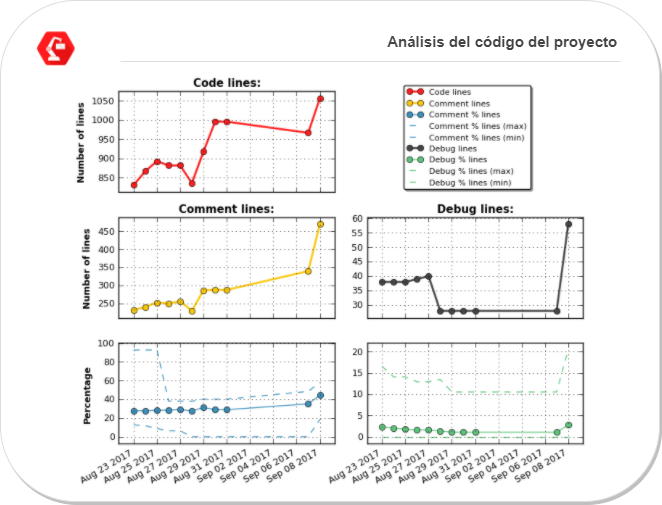
\includegraphics[width=0.75\textwidth]{figuras/SW/analisis_codigo.png}   
        \caption{Análisis del código del proyecto}
        \label{fig:SW:code_analysis}
    \end{figure}
    
